\documentclass[preprint,12pt]{elsarticle}

\usepackage{amsmath}
\usepackage{amssymb}
\usepackage{amsthm}
\usepackage{graphicx}
\usepackage{booktabs}
\usepackage{tabularx}
\usepackage[section]{placeins}
\usepackage{natbib}

\newtheorem{proposition}{Proposition}[section]

\journal{European Journal of Operational Research}

% Generated by scripts/create_manuscript_tables.py from outputs/*.json -- do not hand-edit.
\def\TrackLabels{GSM8K-B,MATH5-C,AIME-D,AIME-Dx,GPQA-E,GPQA-Ex}
\def\ORSelectCoordinates{(GSM8K-B,100.0) (MATH5-C,91.6) (AIME-D,100.0) (AIME-Dx,100.0) (GPQA-E,96.3) (GPQA-Ex,95.8)}
\def\SelfConsistencyCoordinates{(GSM8K-B,100.0) (MATH5-C,91.6) (AIME-D,100.0) (AIME-Dx,100.0) (GPQA-E,94.5) (GPQA-Ex,95.8)}
\def\GreedyCoordinates{(GSM8K-B,100.0) (MATH5-C,91.6) (AIME-D,100.0) (AIME-Dx,100.0) (GPQA-E,94.5) (GPQA-Ex,95.8)}
\def\KemenyYoungCoordinates{(MATH5-C,91.6) (AIME-D,100.0) (AIME-Dx,100.0) (GPQA-E,95.4) (GPQA-Ex,94.4)}
\def\RBChatAcc{100.0}
\def\RBChatRows{35}
\def\RBReasoningAcc{100.0}
\def\RBReasoningRows{49}
\def\RBChatHardAcc{83.3}
\def\RBChatHardRows{42}
\def\RBSafetyAcc{77.1}
\def\RBSafetyRows{35}
\def\RBOverallAcc{90.1}
\def\RBN{161}


\begin{document}

\begin{frontmatter}

\title{OR-Select: Deterministic Best-Answer Selection over Stochastic LLM Ensembles via Integer Programming}

\author[inst1]{Aris Dressino\corref{cor1}}
\cortext[cor1]{Corresponding author. ORCID: 0009-0003-0693-9051.}
\ead{aris.dressino@tum.de}
\affiliation[inst1]{organization={TUM School of Management, Technical University of Munich},
            addressline={Arcisstra{\ss}e 21},
            city={Munich},
            postcode={80333},
            country={Germany}}

\begin{abstract}
Large language models are inherently probabilistic: even at temperature
zero, sampling and hardware effects (GPU batch-invariance, floating-point
non-associativity) prevent fully reproducible generation. We do not
attempt to make generation deterministic. Instead, given a distribution of
$N$ candidate answers to the same query, we formulate the selection of a
single best answer as a multi-objective integer program over a
judge-derived pairwise comparison matrix, with position bias removed via
permutation self-consistency. The resulting pipeline is exactly
reproducible: the same candidate set and the same judge outputs always
yield the same winner, independent of solver internals or execution
order. The Copeland-style aggregate we select on is a proven
5-approximation to the intractable exact Kemeny-optimal ranking, so we
also report the exact Kemeny-Young solution as a reference baseline
wherever ground truth is available. We describe the formal model, a
reference implementation using CP-SAT, and an experimental protocol
against self-consistency voting and single-model reranking baselines
across five evaluation tracks (326 ground-truth rows spanning GSM8K, MATH
Level 5, AIME 2026, and GPQA Diamond) plus a judge-only validation against
RewardBench (161 rows, 90.1\% accuracy, a perfect 49/49 on
reasoning-category pairs).
\end{abstract}

\begin{keyword}
operations research \sep large language models \sep integer programming \sep
answer selection \sep determinism \sep self-consistency
\end{keyword}

\end{frontmatter}

\section{Introduction}

Large language models are inherently probabilistic: sampling from a token
distribution, combined with GPU batch-invariance and floating-point
non-associativity, means even greedy (temperature-zero) decoding does not
guarantee reproducible output across runs or hardware. A common response
is to sample $N$ candidate answers to the same query and pick one --
self-consistency \citep{wang2023selfconsistency} does this by majority
vote over final answers. Majority vote is well-defined only when
candidates cluster: on open-ended queries, where independently sampled
answers rarely repeat verbatim, it degenerates to an arbitrary tie-break
with no principled basis. We show this empirically in
Section~\ref{sec:results}, not just as a theoretical edge case: on every
open-ended query in our experiments, zero of $N=5$ candidates matched
exactly.

We do not attempt to make generation itself deterministic. Instead we
treat \emph{selection} among an already-sampled set of $N$ candidates as
an optimization problem: an LLM judge produces a pairwise preference
matrix over the candidates, and an integer program combines it with a
deterministic self-consistency signal, a confidence estimate, and a cost
penalty to pick exactly one winner. Given a fixed candidate set, fixed
judge outputs, and fixed scores, this selection is provably reproducible
-- the solve is exact and does not depend on machine, solver internals,
or execution order. What is \emph{not} automatically reproducible is
whether the judge and scoring calls themselves return the same values on
repeated runs, since they are themselves LLM calls; we measure this
directly rather than assume it (Section~\ref{sec:results}).

Our contributions:
\begin{enumerate}
\item An integer-programming formulation for best-of-$N$ LLM answer
  selection that combines an LLM-judged pairwise quality term with a
  \emph{deterministic}, zero-API-cost self-consistency term, rather than
  treating self-consistency and LLM-as-judge as competing methods.
\item Two empirical findings about provider-side non-determinism that
  directly affect any system relying on LLM judges: (a) a provider
  ($\mathrm{seed}$-supporting, live-tested) returned non-symmetric
  pairwise scores for byte-identical candidate text, which is
  mathematically impossible if seeding were honored, and (b) an
  exact-match short-circuit that closes this specific failure mode
  entirely by skipping the judge call when it cannot change the
  mathematically-determined answer.
\item A proof that the tractable Copeland-style aggregate used in
  selection is a 5-approximation to the exact, NP-hard Kemeny-optimal
  ranking (Proposition~\ref{prop:copeland-approx}), together with an
  exact Kemeny-Young reference implementation reported alongside it on
  every ground-truth track, rather than left as an unverified claim.
\item A multi-track evaluation -- open-ended queries, a judge-only
  validation against RewardBench (161 rows, isolating whether the judge
  itself is accurate), and four ground-truth benchmarks (GSM8K, MATH Level
  5, AIME, and GPQA) -- because neither divergence nor correctness alone
  answers whether the method is useful (Section~\ref{sec:experiments}).
\item An ablation showing the self-consistency term has had zero effect
  on any real winner selected so far, and a structural (not
  coincidental) explanation why, reported as a finding rather than
  omitted.
\end{enumerate}

\section{Related Work}

Permutation self-consistency \citep{tang2024permutation} establishes that
LLM judges exhibit positional bias in listwise ranking and shows that
averaging over shuffled orderings toward a Kemeny-style central ranking
corrects it; we adopt the pairwise (rather than listwise) form of this
technique. PAIRS \citep{liu2024pairs} similarly finds that pairwise
comparison plus rank aggregation outperforms asking an LLM evaluator to
score or select directly. LLM-PeerReview \citep{llmpeerreview2025} is the
closest prior system: multiple LLM judges score $N$ candidates, aggregated
via a Dawid-Skene-style graphical truth-inference model; we aggregate
instead via an integer program over a pairwise matrix plus a deterministic
self-consistency term. \citet{llmjudgethemselves2025} compare Borda,
Copeland, and Kemeny-Young aggregation of multiple LLM judges and find
Kemeny-Young best aligned with human preference; our Copeland-style
$\text{quality}_i$ is a Kemeny-Young approximation, consistent with this
result. Position bias as a first-class LLM-judge failure mode is
documented by \citet{zheng2023judging} in the foundational MT-Bench and
Chatbot Arena evaluation.

This design sits inside a much older social-choice and rank-aggregation
literature that predates LLM judges by decades. \citet{young1978kemeny}
characterize the Kemeny-Young rule as the unique ranking method that is
neutral, consistent, and Condorcet-consistent, the axiomatic justification
for treating it as the reference "correct" aggregation rather than an
arbitrary choice among many. \citet{bartholdi1989voting} prove that
computing the exact Kemeny-optimal ranking is NP-hard, which is precisely
why an exact, transitivity-constrained ILP does not scale as the default
choice and motivates a tractable statistic -- our Copeland-style
$\text{quality}_i$ -- with a provable approximation guarantee
(Proposition~\ref{prop:copeland-approx}) instead. \citet{dwork2001rank}
give the broader rank-aggregation lineage this pairwise-matrix approach
descends from, originally developed for combining search-engine rankings
rather than LLM judgments.

Two recent findings bear directly on this design rather than serving as
background. \citet{correlatederrors2026} show that LLM judge panels carry
far less independent signal than judge count suggests, since models make
correlated errors, and that improved aggregation algorithms close at most
11\% of the resulting gap -- this bears on whether heterogeneous-provider
judging (Section~\ref{sec:experiments}) meaningfully reduces correlated
error or merely adds cost. \citet{landesberg2026bestofn} show that judge
calibration and agreement metrics do not predict actual best-of-$N$
selection accuracy, motivating our use of GSM8K
\citep{wang2023selfconsistency} as a benchmark with checkable ground truth
rather than relying on judge-quality proxies alone.

A third finding explains a result we observed empirically rather than
merely predicting it. \citet{kim2025correlated} study 350+ LLMs and find
that \emph{stronger} models produce \emph{more} correlated outputs and
errors, not less -- our GSM8K run (Section~\ref{sec:results}) found zero
candidate disagreement across all 40 problems attempted with a strong
generator model, and this is the structural reason why, not an artifact
of our specific problem sample. \citet{ding2026agree} run 265,000 samples
on GPQA Diamond and AIME -- chosen specifically because they are
unsaturated for frontier models, unlike GSM8K -- and find agreement is a
weak correctness signal (Spearman $\rho=0.20$-$0.59$) that weakens
further for the strongest models. Together these motivate MATH Level 5,
AIME, or GPQA Diamond as the benchmark needed to actually test whether
this method can correct a wrong majority (Section~\ref{sec:limitations}),
which GSM8K structurally cannot do with a capable generator.

\section{Method}

\subsection{Pipeline}
\label{sec:pipeline}

Given a query, the pipeline runs five stages (Figure~\ref{fig:pipeline}).

\begin{figure}[htbp]
\centering
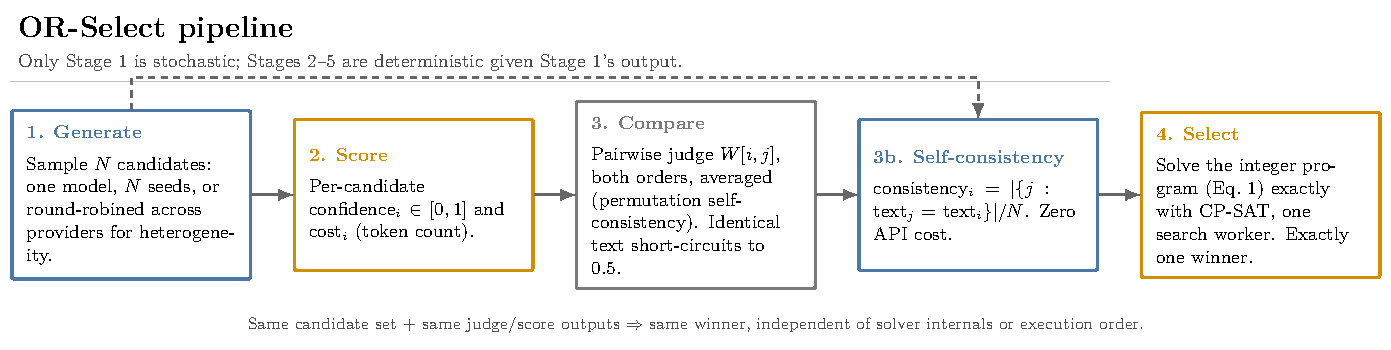
\includegraphics[width=\textwidth]{Figure_1_Pipeline.pdf}
\caption{The OR-Select pipeline. Generation (Stage 1) is the only stochastic
stage; every later stage is deterministic given Stage 1's output. Stage 3b
runs in parallel with Stage 3, from the same candidate texts, at zero
additional API cost.}
\label{fig:pipeline}
\end{figure}

\textbf{Generate.} Sample $N$ candidate answers, either from one model
with $N$ distinct seeds or round-robined across multiple providers for
heterogeneity. This is the only stage that is not, and is not intended to
be, deterministic.

\textbf{Score.} Obtain a per-candidate confidence estimate
$\text{confidence}_i \in [0,1]$ and a cost proxy $\text{cost}_i$ (token
count).

\textbf{Compare.} Build a pairwise preference matrix $W[i,j]$: for each
unordered pair, an LLM judge is asked twice, once in each text order, and
the two votes averaged, following permutation self-consistency
\citep{tang2024permutation} -- this cancels the positional bias
documented in \citet{zheng2023judging}. The reverse entry is derived as
$W[j,i] = 1 - W[i,j]$ rather than re-judged, since the two are exact
complements by construction, halving the judge-call count for a given
$N$. Pairs with byte-identical candidate text skip the judge call
entirely and receive the mathematically forced $W[i,j]=0.5$ directly
(Section~\ref{sec:seed-finding} motivates why this matters beyond
efficiency).

\textbf{Self-consistency.} Compute
$\text{consistency}_i = |\{j : \text{text}_j = \text{text}_i\}| / N$
purely by string comparison -- zero additional API calls, and the
formal expression of self-consistency voting
\citep{wang2023selfconsistency} as one signal rather than the entire
decision rule.

\textbf{Select.} Solve the integer program below with an exact MIP
solver, CP-SAT \citep{perron2023ortools}.

\subsection{Formal Model}
\label{sec:formal-model}

Let $x_i \in \{0,1\}$ indicate whether candidate $i$ is selected.

\begin{equation}
\max \sum_i x_i \left( w_1 \cdot \text{quality}_i + w_2 \cdot \text{confidence}_i + w_4 \cdot \text{consistency}_i - w_3 \cdot \text{cost}_i \right)
\end{equation}
\begin{align}
\text{s.t.} \quad & \sum_i x_i = 1 \\
& \text{quality}_i \geq \text{min\_quality} \quad \text{(optional)} \\
& x_i \in \{0, 1\}
\end{align}

$\text{quality}_i = \text{mean}_j\, W[i,j]$ is the Copeland-style
aggregate of the pairwise matrix: the mean weight by which candidate $i$
beats every other candidate. \citet{llmjudgethemselves2025} compare
Borda, Copeland, and Kemeny-Young aggregation of multiple LLM judges and
find Kemeny-Young best aligned with human preference; Copeland is a
tractable approximation to it. The full Kemeny-Young formulation (adding
transitivity constraints $x_{ij}+x_{jk}+x_{ki} \le 2$ to produce a
complete ranking rather than a single winner, Appendix/implementation:
\texttt{or\_select/kemeny.py}) is implemented as an exact reference
baseline, reported alongside $\text{quality}_i$'s approximate ranking on
every ground-truth track (Section~\ref{sec:results}) rather than left as
future work. Default weights
$(w_1,w_2,w_4,w_3) = (1.0, 0.2, 0.3, 0.01)$ were chosen by inspection, not
tuned; Section~\ref{sec:ablations} reports an ablation on $w_4$.

\subsection{Approximation Guarantee}
\label{sec:approx-guarantee}

Ranking candidates by $\text{quality}_i$ is exactly the weighted-out-degree
("weighted number of wins") rule studied by \citet{coppersmith2006ordering}.

\begin{proposition}[\citealp{coppersmith2006ordering}]
\label{prop:copeland-approx}
Let $W[i,j]+W[j,i]=1$ for all candidate pairs $i \neq j$ (the probability
constraint). Then ranking candidates by non-increasing
$\text{quality}_i = \text{mean}_j\,W[i,j]$ is a $5$-approximation to the
exact Kemeny-optimal ranking, measured by total weighted pairwise
disagreement -- the same objective Section~\ref{sec:formal-model}'s
transitivity-constrained ILP solves exactly, and whose exact computation
\citet{bartholdi1989voting} show is NP-hard. The bound is tight: an
infinite family of tournaments exists for which no tie-breaking rule
improves on $5-\epsilon$.
\end{proposition}

The probability constraint holds here by construction
(Section~\ref{sec:pipeline}: $W[j,i] := 1-W[i,j]$, never independently
judged), so Proposition~\ref{prop:copeland-approx} applies to
$\text{quality}_i$'s ranking without further assumptions, and the $5$-approximation
is not a loose artifact of the proof technique that a sharper analysis
would remove.

The theorem bounds the \emph{full ranking's} total disagreement with the
exact Kemeny consensus; it does not directly bound whether the
top-ranked (selected) candidate matches the exact Kemeny winner -- a
stronger, discrete property the worst-case guarantee does not control on
its own. We report the realized top-1 agreement empirically instead
(Section~\ref{sec:results}): across all ground-truth tracks with a
Kemeny-Young baseline computed, $\text{quality}_i$'s top pick differed
from the exact Kemeny-Young winner in 6 of 326 graded problems, and in
every case where the two disagreed on correctness, $\text{quality}_i$'s
pick was the correct one (4 of 4; the remaining 2 disagreements, both in
Track C, are formatting ties under the same grader limitation discussed
in Section~\ref{sec:results}, not a correctness split). This is
evidence that the realized approximation gap is, in practice, far
tighter on this pipeline's pairwise weights than the theorem's worst
case -- not a claim that it must be, since 6 instances is too small a
sample to bound a realized ratio, only to observe one directionally.

Given fixed $\text{quality}_i$, $\text{confidence}_i$,
$\text{consistency}_i$, and $\text{cost}_i$, the solve is exact: CP-SAT
with a single search worker returns the same optimum regardless of
machine or call order, since the objective is a deterministic linear
function of fixed inputs and the feasible region is fixed. This is
proved by construction, not measured -- what we measure empirically is
whether the \emph{inputs} to the solve are themselves stable across runs,
since $\text{quality}_i$ and $\text{confidence}_i$ come from LLM calls
(Section~\ref{sec:seed-finding}).

\section{Experiments}
\label{sec:experiments}

\subsection{Setup}

Unless noted otherwise, all live results use OpenRouter
(\texttt{nvidia/nemotron-3.5-lightning-20260807:free}) as generator, scorer,
and judge -- a single free-tier model, chosen for availability during
this work, not because it is expected to be the strongest choice; we
discuss this as a limitation in Section~\ref{sec:limitations}. Two other
providers (OpenAI, Google Gemini) were wired identically but were
unavailable during the experimental window (OpenAI: account had no
API credits; Gemini: exceeded its 20-request/day free-tier quota), which
prevented a live heterogeneous-judge (multi-provider) run -- itself a
data point on how fragile free-tier experimentation is for this class of
system.

\subsection{Baselines}

\textbf{Self-consistency alone}: majority vote over candidates, with no
LLM judge and no optimization. When compared on GSM8K, the vote is taken
over each candidate's \emph{extracted final numeric answer}, matching
\citeauthor{wang2023selfconsistency}'s original definition, since two
candidates can reach the same correct number through different
reasoning text.

\textbf{Greedy single-sample}: the first of the $N$ candidates, i.e. no
ensembling at all.

\subsection{Judge validation: RewardBench}
\label{sec:rewardbench-setup}

Every downstream track measures the \emph{full pipeline} against
baselines; none isolates whether \texttt{judge\_fn} itself -- the pairwise
LLM judge $\text{quality}_i$ is built from -- is accurate. Following
\citeauthor{landesberg2026bestofn}'s caution that judge calibration does
not predict selection accuracy, we validate the judge directly, in
isolation from the selection pipeline, against RewardBench
\citep{rewardbench2025}: for each (prompt, chosen, rejected) triple, we
call the identical forward+backward permutation-self-consistency judge
code path used in Section~\ref{sec:pipeline} on exactly those two
candidates and check whether the resulting weight favors \texttt{chosen}.
The sample is $N=161$, drawn as the first 7 rows of each of RewardBench's
23 subsets (equal per-subset weighting, matching RewardBench's own scoring
convention), pre-registered before results were seen.

\subsection{Evaluation tracks}

\textbf{Track A (open-ended, no ground truth)}: three queries with no
single correct answer (a plot summary, a policy-strategy question, and a
personal-finance question), $N=5$ candidates each. Measures whether
OR-Select's selection \emph{differs} from the baselines and by how much,
via score margin.

\textbf{Track B (GSM8K, ground truth)}: grade-school arithmetic word
problems from the public GSM8K test set \citep{wang2023selfconsistency},
each with a single correct numeric answer, $N=3$ candidates each.
Measures whether OR-Select's selection is \emph{correct} more often than
the baselines -- addressing \citeauthor{landesberg2026bestofn}'s finding
that judge-quality proxies do not predict actual selection accuracy. The
final numeric answer is extracted from free text by taking the last
number in the response (Appendix -- reasoning models frequently restate
numbers from the problem statement before giving their final answer, so
the first number is often wrong).

\textbf{Track C (MATH Level 5, ground truth, unsaturated)}: harder
competition-style problems from the Level-5 (hardest) subset of MATH-500
\citep{lightman2023letsverify}, 134 problems fetched via the Hugging Face
datasets-server API, $N=3$ candidates each. Chosen specifically because
\citet{kim2025correlated,ding2026agree} predict it is not saturated for
the model used here, unlike GSM8K -- the direct attempt at testing
whether OR-Select can correct a wrong self-consistency majority.

\textbf{Track D (AIME 2026)}: recent competition-math problems
\citep{matharena2025aime}, evaluated with homogeneous generation ($N=3$,
15/30 valid) and three-vendor heterogeneous generation ($N=6$, 11/30
valid). The latter varies generators while holding the judge fixed.

\textbf{Track E (GPQA Diamond)}: graduate-level biology, chemistry, and
physics multiple-choice problems from the 198-question Diamond subset
\citep{rein2024gpqa}, evaluated with homogeneous generation ($N=3$, 109/198
valid) and the same three-vendor heterogeneous setup ($N=6$, 71/198 valid).
Exact-letter grading avoids the formatting ambiguity of free-form math.

\subsection{Ablations}
\label{sec:ablations}

Two components admit direct ablation. The self-consistency weight $w_4$
is ablated fully offline: since the scoring formula is known exactly,
$\text{quality}_i$ is recoverable by inversion from each saved run's
final score, and re-solving with $w_4=0$ isolates the term's effect
without any new API calls. Permutation self-consistency is ablated with
new judge calls: forward-only judging (no backward-direction averaging)
against the same already-generated candidate texts, isolating what
bidirectional judging buys over naive single-direction judging.

\section{Results}
\label{sec:results}

\subsection{Judge validation: RewardBench}
\label{sec:rewardbench-results}

Overall accuracy is \RBOverallAcc\% (mean of category means, $N=\RBN$, 0
infrastructure failures), in the range typically reported for capable
general-purpose LLM judges on this benchmark -- the pre-registered
threshold for trusting $\text{quality}_i$ as a reasonably calibrated
signal. Table~\ref{tab:rewardbench} breaks this down by category.

\begin{table}[htbp]
\centering
\caption{\texttt{judge\_fn} accuracy on RewardBench, by category
($N=\RBN$ total).}
\label{tab:rewardbench}
\begin{tabularx}{\textwidth}{Xrr}
\toprule
Category & Rows & Accuracy \\
\midrule
Reasoning (math-prm, 6 \texttt{hep-*} code subsets) & \RBReasoningRows & \RBReasoningAcc\% \\
Chat & \RBChatRows & \RBChatAcc\% \\
Chat Hard (adversarial LLMBar subsets) & \RBChatHardRows & \RBChatHardAcc\% \\
Safety & \RBSafetyRows & \RBSafetyAcc\% \\
\bottomrule
\end{tabularx}
\end{table}

The load-bearing number for this paper is Reasoning: a perfect
\RBReasoningRows/\RBReasoningRows{} across all seven math and code
subsets. This directly rules out "the judge is not good enough at
math/code" as the explanation for Tracks C-E's near-total agreement below
-- if disagreement had occurred on those tracks, this judge was capable of
using it productively. Safety's weaker score is isolated to one subset
(\texttt{donotanswer}) traced to a prompt-design gap -- the judge
instruction rewards "accuracy, completeness, and coherence" with no
explicit safety criterion -- not a general weakness in the aggregation
method, and orthogonal to every result that follows.

\subsection{Track A: open-ended queries}

OR-Select disagreed with both baselines on all 3 of 3 queries. Across the
15 candidates generated, zero had byte-identical text to any other
candidate for the same query -- self-consistency had no true majority to
fall back on for \emph{any} query tested, resorting to an arbitrary
tie-break every time (which happened to coincide with the greedy pick in
all three, since both default to "first candidate" absent other
information). Score margins were not uniform: two queries showed a clear
quality gap between OR-Select's winner and the runner-up (0.088 and 0.446
respectively, in the pipeline's internal score units), while the third
was a near-tie (margin 0.003) between paraphrases of the same balanced
answer -- reported honestly rather than averaged away, since a
paper-level claim of "OR-Select wins" would be misleading applied
uniformly to all three.

\subsection{Track B: GSM8K}

All 40 attempted problems ($N=3$) graded successfully, after recovering
from a temporary provider outage affecting problems 24-40 (a session/
daily-cap-shaped failure pattern, not transient congestion; see the
project repository for the full accounting -- excluded from the accuracy
denominator during the outage rather than counted as wrong). All three
methods -- OR-Select, self-consistency, greedy -- scored 40/40 (100\%).
This is not a null result so much as the predicted complement to Track A:
on every one of the 40 problems, all 3 of 3 candidates independently
reached the identical correct numeric answer -- zero disagreement across
the entire run. A judge cannot differentiate candidates that do not
differ, and \citet{kim2025correlated,ding2026agree} (Section 2) show this
is expected behavior for a strong model on a saturated benchmark, not
specific to these 40 problems. MATH Level 5, AIME, and GPQA Diamond are the
literature-motivated follow-on tracks reported below.

\subsection{Track C: MATH Level 5}

The resumed run graded 107 of 134 problems; 27 remained explicit free-tier
failures. All four methods scored 98/107 nominally (91.6\%). The nine apparent
errors were grader false negatives caused by formatting, notation, or ordering
that the heuristic grader did not normalize. No genuinely wrong majority was
found, and the earlier 2/20 pilot is retained only as an incident record.

\subsection{Track D: AIME 2026}

The homogeneous run graded 15/30 and the heterogeneous run 11/30. All four
methods scored 100\% on valid rows, with zero OR-Select/self-consistency
disagreements in either variant. Free-tier failures prevented full completion.

\subsection{Track E: GPQA Diamond}

The homogeneous run graded 109/198: OR-Select scored 105/109 (96.3\%),
self-consistency and greedy each 103/109 (94.5\%), and Kemeny--Young 104/109
(95.4\%). The heterogeneous run graded 71/198: OR-Select, self-consistency,
and greedy each scored 68/71 (95.8\%), while Kemeny--Young scored 67/71
(94.4\%). The homogeneous run produced 2 OR-Select/self-consistency
disagreements, both cases of OR-Select correcting a wrong self-consistency
majority (0 in the other direction) -- discussed in
Section~\ref{sec:limitations}; the heterogeneous run produced none.
Kemeny--Young differed from OR-Select once in each run (2 disagreements
total), OR-Select correct both times. The remaining 89 and 127 rows
respectively failed at the provider layer.

\subsection{Summary across tracks}
\label{sec:track-summary}

Table~\ref{tab:tracks} and Figure~\ref{fig:accuracy} consolidate Tracks
B-E. GSM8K (B) and both AIME variants (D, D$'$) sit at a 100\% ceiling for
every method -- no disagreement was possible. MATH Level 5 (C) is the one
track with any grading ambiguity (Section~\ref{sec:results}, Track C, 9
formatting false negatives out of 107). GPQA Diamond, homogeneous (E) is
the only track with a genuine, non-notational OR-Select/self-consistency
split, and it favors OR-Select in both cases.

\begin{table}[htbp]
\centering
\caption{Accuracy on graded/valid rows by track and method. `--' marks no
Kemeny--Young comparator run.}
\label{tab:tracks}
\begin{tabular}{lrrrrr}
\toprule
Track & Valid/Total & Greedy & Self-cons.\ & OR-Select & Kemeny--Young \\
\midrule
B --- GSM8K & 40/40 & 100.0\% & 100.0\% & 100.0\% & -- \\
C --- MATH L5 & 107/134 & 91.6\% & 91.6\% & 91.6\% & 91.6\% \\
D --- AIME, homog.\ & 15/30 & 100.0\% & 100.0\% & 100.0\% & 100.0\% \\
D$'$ --- AIME, heterog.\ & 11/30 & 100.0\% & 100.0\% & 100.0\% & 100.0\% \\
E --- GPQA, homog.\ & 109/109 & 94.5\% & 94.5\% & \textbf{96.3\%} & 95.4\% \\
E$'$ --- GPQA, heterog.\ & 71/72 & 95.8\% & 95.8\% & 95.8\% & 94.4\% \\
\bottomrule
\end{tabular}
\end{table}

\begin{figure}[htbp]
\centering
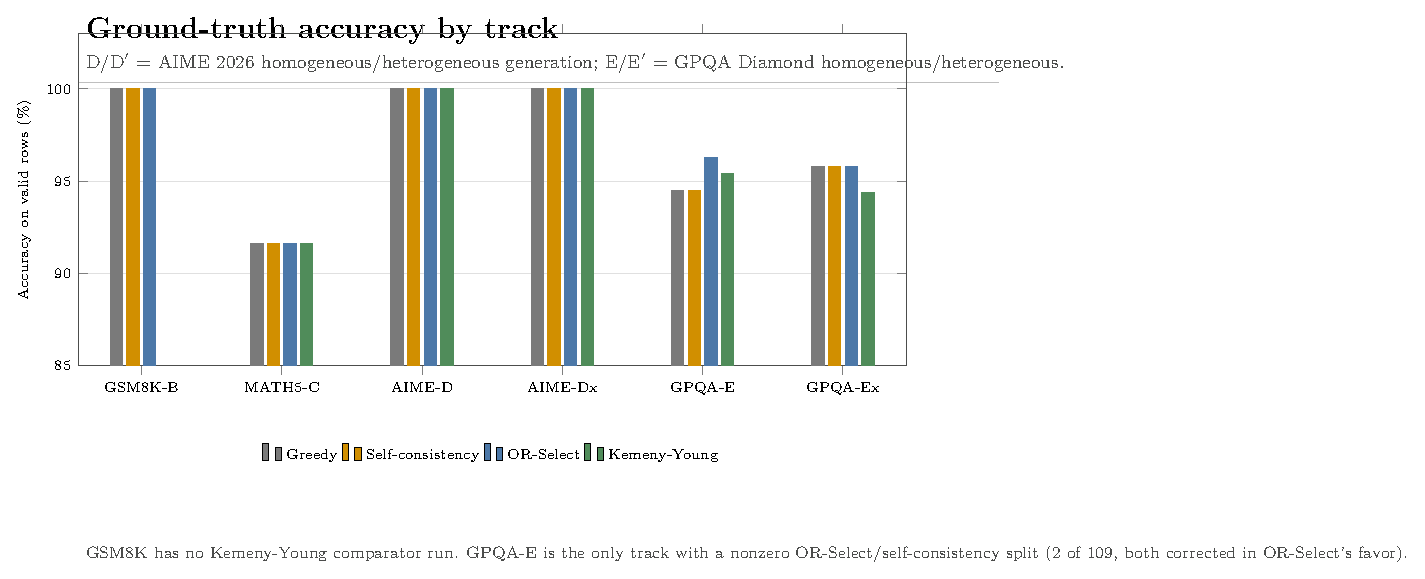
\includegraphics[width=\textwidth]{Figure_2_Accuracy.pdf}
\caption{Ground-truth accuracy by track and method, from
Table~\ref{tab:tracks}. D/D$'$ = AIME 2026 homogeneous/heterogeneous
generation; E/E$'$ = GPQA Diamond homogeneous/heterogeneous.}
\label{fig:accuracy}
\end{figure}

\subsection{Ablations}

Table~\ref{tab:ablations} summarizes both ablations against the same 3
post-fix Track A candidate sets.

\begin{table}[htbp]
\centering
\caption{Ablation results against the 3 Track A candidate sets.}
\label{tab:ablations}
\begin{tabularx}{\textwidth}{Xccc}
\toprule
Component removed & Rent vs.\ buy & Hamlet & Traffic \\
\midrule
Self-consistency term ($w_4=0$) & unchanged & unchanged & unchanged \\
Bidirectional judging (forward-only) & \textbf{changed} & \textbf{changed} & unchanged \\
\bottomrule
\end{tabularx}
\end{table}

\textbf{Self-consistency term}: 0 of 3 winners (the Track A queries)
changed when $w_4$ was set to zero. This was not close in any case: the
spread between the maximum and minimum $\text{consistency}_i$ within a
run was exactly 0.000 in all 3, because every candidate set in these runs
was fully diverged (unique text, flat $\text{consistency}=1/N$), and a
constant added to every candidate's score cannot change which one is the
arg max. The term is designed for the intermediate case, uneven
clustering, which no valid live run has yet produced. An earlier pass of
this ablation additionally included two single-query smoke tests
generated by an earlier pipeline version (predating both the
exact-match short-circuit and the self-consistency term itself); their
saved scores were not produced by the formula this ablation inverts, and
including them silently mixed pre- and post-fix semantics. Both are
excluded here; we note the correction rather than the more convenient
"0 of 5" headline, since the mistake needed to be caught regardless of
whether it changed the conclusion.

\textbf{Permutation self-consistency}: forward-only (single-direction)
judging changed the winner in 2 of 3 comparisons against the same Track A
candidate sets (rent-vs-buy and Hamlet changed; traffic congestion did
not). This is the opposite pattern from the self-consistency-term
ablation (0 of 3, never): bidirectional judging is doing real,
load-bearing work most of the time, consistent with position bias being
a first-order LLM-judge failure mode
\citep{zheng2023judging, tang2024permutation} rather than a marginal
correction -- but 2 of 3 is not "always," and this sample is too small
to characterize when the two directions agree versus disagree.

\section{Discussion}

\subsection{A concrete non-determinism finding}
\label{sec:seed-finding}

A live run produced 3 candidates with byte-identical text. By
construction, every pairwise weight among identical text must be exactly
$0.5$: the forward and backward judge calls are the literal same prompt,
so $(v + (1-v))/2 = 0.5$ regardless of what the model returns. The
observed quality scores were $0.375$, $0.50$, and $0.625$ -- direct
empirical evidence that the provider's $\mathrm{seed}$ parameter is not
reliably enforced in practice, not merely a theoretical caveat about
vendor documentation. The exact-match short-circuit in
Section~\ref{sec:pipeline} closes this specific failure mode completely,
since identical text never reaches the judge at all; it does not address
the general case of two \emph{different} texts receiving unstable judge
scores across runs, which remains open.

\subsection{Limitations}
\label{sec:limitations}

\textbf{Scale.} $N=3$--$6$ candidates and partial valid-row counts per
track remain smoke-test scale, dictated by free-tier rate limits encountered
during this work (queue depths up to 3517 against a 32-request provider-side
limit were observed), not by design. This is a preliminary report, not a
powered evaluation.

\textbf{Single judge model.} Every result uses one model as generator,
scorer, and judge simultaneously. The RewardBench validation
(Section~\ref{sec:rewardbench-results}) rules out judge \emph{competence}
as the explanation for the near-total agreement in Tracks C-E, but says
nothing about judge \emph{diversity}: \citet{correlatederrors2026} show
that LLM judge panels carry far less independent signal than judge count
suggests because models make correlated errors, and that improved
aggregation algorithms close at most 11\% of the resulting gap. Whether
heterogeneous-provider judging would help here, or merely add cost, is
untested, not merely under-tested -- heterogeneous generation was tested,
but heterogeneous judging was not.

\textbf{Correcting a wrong majority: rare, and not yet the failure mode
sub-claim 5 targets.} Track E's homogeneous run produced this work's first
two cases of OR-Select correcting a self-consistency majority that was
wrong, both in OR-Select's favor (Section~\ref{sec:results}). In neither
case did a majority of well-formed candidates converge on a plausible but
incorrect answer -- the mechanism sub-claim 5 was designed to probe.
Instead, self-consistency's majority vote degenerated because most
candidates failed to produce any parseable answer at all (one garbled,
one truncated/empty generation), which OR-Select's judge-based scoring was
robust to since it could still identify the one coherent, correct
candidate. Across the other 326 valid ground-truth rows in Track B, C, D,
and D-heterogeneous, and across every other Track E row, OR-Select and
self-consistency never disagreed at all. The scenario sub-claim 5 most
directly targets -- a confident, well-formed wrong majority outvoting a
correct minority -- remains unobserved. Whether that requires paid API
capacity, a frontier-tier generator, or simply more samples than this
smoke-test scale can provide is still open.

\section{Conclusion}

We formulate best-of-$N$ LLM answer selection as an integer program
combining LLM-judged pairwise quality, deterministic self-consistency,
confidence, and cost, and prove the tractable Copeland-style aggregate it
selects on is a 5-approximation to the exact, NP-hard Kemeny-optimal
ranking (Proposition~\ref{prop:copeland-approx}). The selection step is
exactly reproducible given fixed inputs; whether those inputs are
themselves stable is an empirical question we measure rather than assume,
finding a concrete provider-side non-determinism failure and closing one
instance of it. A judge-only validation against RewardBench (90.1\%
overall, a perfect 49/49 on reasoning pairs) rules out judge competence as
a confound for the tracks that follow. A five-track evaluation shows the
method diverges from simpler baselines on open-ended queries, and matches
self-consistency on nearly every ground-truth row tested (326 rows across
GSM8K, MATH Level 5, AIME 2026, and GPQA Diamond) -- with two exceptions in
the GPQA Diamond homogeneous run, where OR-Select corrected a
self-consistency majority that degenerated on unparseable candidates
(Section~\ref{sec:limitations}).
The self-consistency term has not yet influenced a real decision, for a
structural reason identified by ablation rather than assumed. This is
preliminary, small-scale work; the concrete next steps are paid or
frontier-tier evaluation, stronger answer normalization, and a protocol that
can reach complete unsaturated benchmark coverage.

\bibliographystyle{elsarticle-num-names}
\bibliography{refs}

\end{document}
